\documentclass[JohnsonMADraft3]{subfiles}
\begin{document}
\doublespacing

I have specified two different models.  A primary specification with five indicators and 42 years of data and a regime change specification consisting of regime change observations over 200 years with four indicators.

Each model was run in R using Martyn \citeauthor{r-rjags}'s JAGS package and the CODA package for convergence diagnostics \cite{R,r-CODA}.\footnote{Other software packages used are listed in the Reference section without being cited in-text.}  Convergence is assessed using the Gelman-Rubin Diagnostic procedure \citeauthor{r-superdiag}'s \textit{Superdiag} package in R \citep{Gelman1992,R}.

%Software Citations
\nocite{R,r-CODA,r-Foreign,r-R2jags,r-ggplot2,r-dplyr,r-rjagsr-doParallel,r-rcurl,r-random,r-superdiag,r-polycor}

%\subsection{Primary Specification}
The primary model is composed of all state year observations between 1800 and 2012.  There are four indicators in this model: Appointment Method, Initial Term Length, Subsequent Term Length and Retention Method.  There are 8,436 state-year observations.  

Figure \ref{continuumresults} shows how the results from this model map on to the Independence Continuum discussed in Section \ref{Theory}

\todo{Update this with results from model}\begin{figure}[tbh]\centering\caption{Independence Continuum}\label{continuumresults}
	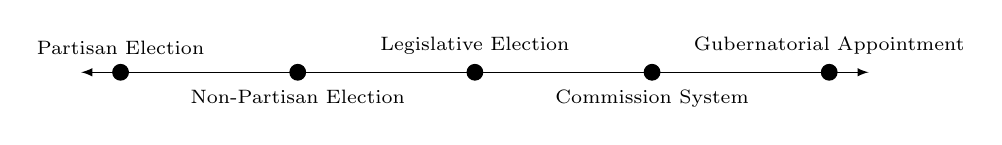
\begin{tikzpicture}
	% a straight line segment
	\draw[latex-latex] (-0.5,0) -- (9.5,0);
	%% the labels
	\node[fill=black,draw=black,circle,inner sep=2pt,label=above:{\scriptsize Gubernatorial Appointment}] at (9,0) {};
	\node[fill=black,draw=black,circle,inner
	sep=2pt,label=below:{\scriptsize Commission System}] at (6.75,0) {};
	\node[fill=black,draw=black,circle,inner
	sep=2pt,label=above:{\scriptsize Legislative Election}] at (4.5,0) {};
	\node[fill=black,draw=black,circle,inner
	sep=2pt,label=below:{\scriptsize Non-Partisan Election}] at (2.25,0) {};
	\node[fill=black,draw=black,circle,inner sep=2pt,label=above:{\scriptsize Partisan Election}] at (0,0) {};
	\end{tikzpicture}
\end{figure} 

\subsection{Five Indicator Specification}
The Five Indicator specification of this model is composed of all state year observations from 1970-2012. There are five indicators in this specification, the same four in the primary specification, with the addition of the indicator for docket control.  

\begin{figure}
\centering
\caption{Five Indicator Specification- Additive vs. IRT}
\label{fig:fiveind_additive_ggplot}
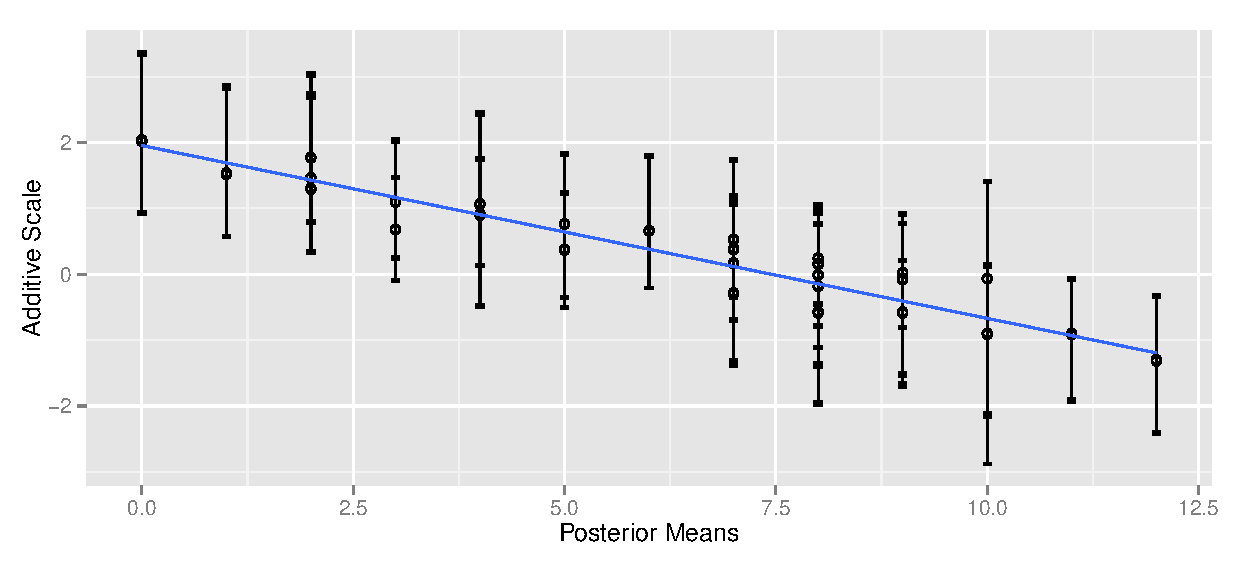
\includegraphics[width=0.7\linewidth]{graphics/fiveind/fiveind_additive_ggplot}
\end{figure}

Figure \ref{fig:fiveind_additive_ggplot} shows the results of an additive scale for the relevant indicators and data in the alternative specification.  The Pearson's Correlation between the additive and the IRT model is $-.9553$ \todo{Update this with new value} with a $p$-value of $<.001$.

\subsection{Regime Change Specification}
The second model specification consists of the four original indicators, but is limited to only unique observations of each judicial institution rather than repeated observations over long periods of time.  This specification dramatically reduces the number of observations.  For instance, Massachusetts, which has maintained the same selection/retention methods as well as the same term lengths for its entire history has only a single observation.  There are 155 state-year observations in this model specification.  The Regime Change Specification was run using 10,000 draws with the first 5,000 thrown away as burnin.  Convergence was assessed with a Gelman-Rubin Diagnostic, with a Multivariate Potential Scale Reduction Factor of 1.04 \citep{Gelman1992}.  

\begin{figure}
\centering
\caption{Regime Specification- Additive vs. IRT}
\label{fig:regime_additive_ggplot.pdf}
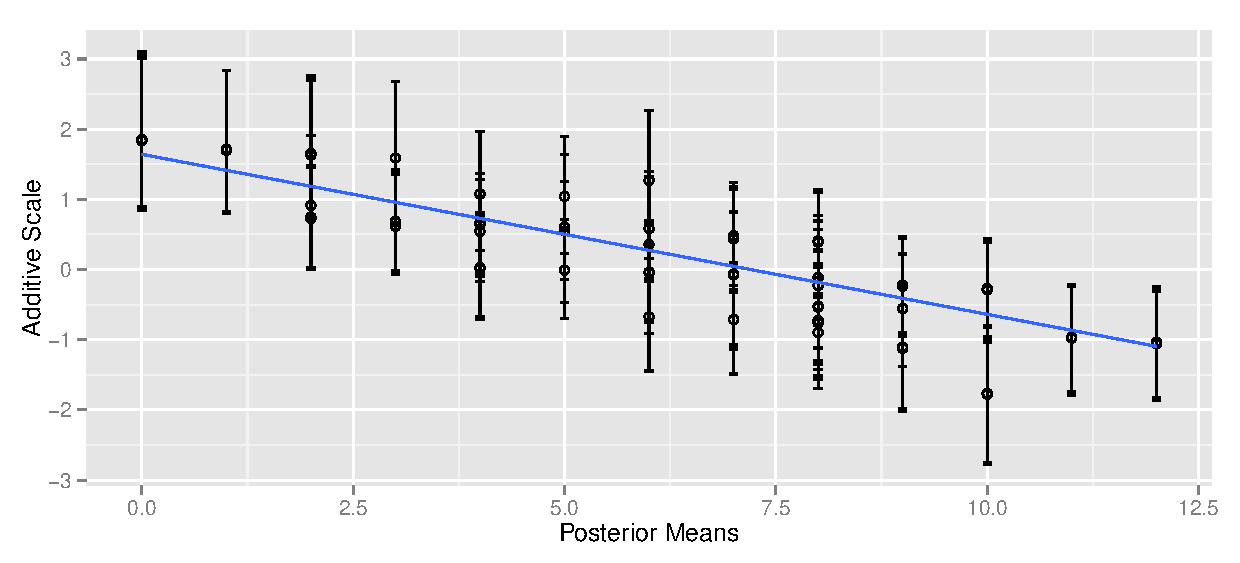
\includegraphics[width=0.7\linewidth]{graphics/regime/regime_additive_ggplot}
\end{figure}

Figure \ref{fig:regime_additive_ggplot} shows the results of an additive scale for the relevant indicators in the Regime Change specification plotted against the IRT model.  The Pearson's Correlation between the additive model and the IRT model is $-.899$, with a $p$-value of $>.001$.

\begin{figure}
	\centering	\caption{Regime Change Specification- Parameter Means}\label{regime_parametermean}
	\begin{subfigure}{.5\textwidth}
		\centering
		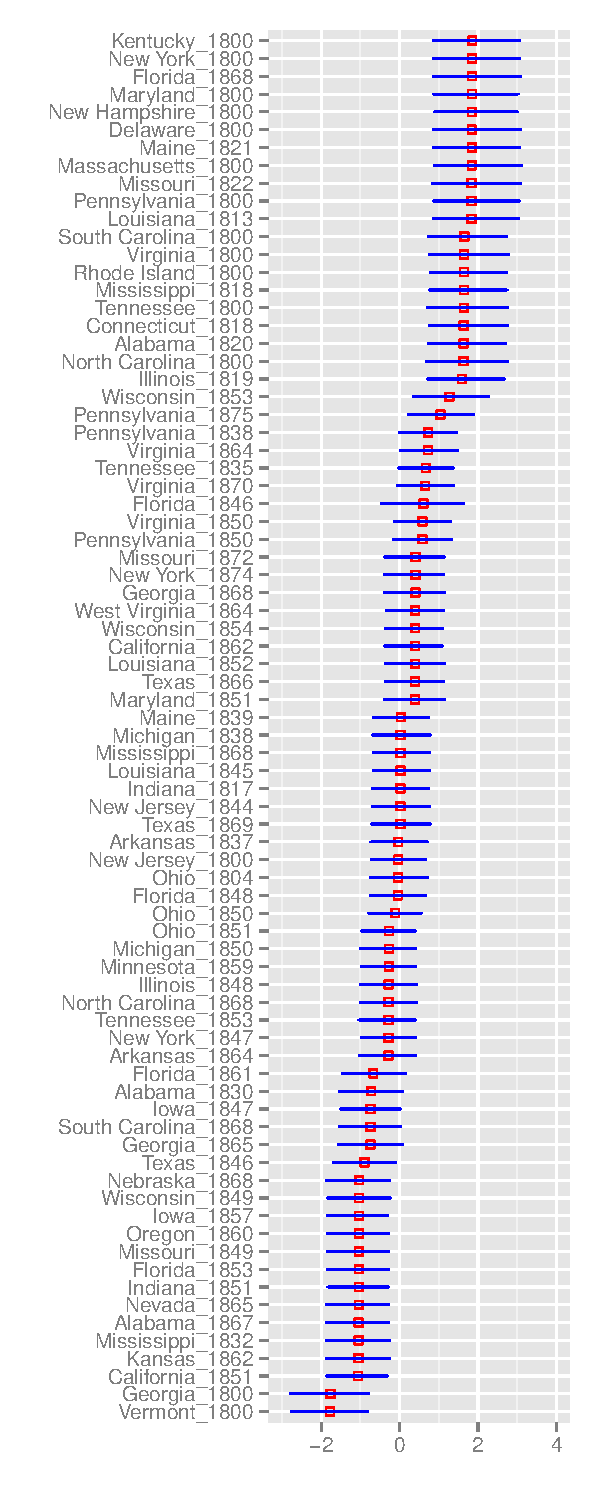
\includegraphics[height=\textheight]{graphics/regime/regime_param_mean_first_ggplot.pdf}
		\end{subfigure}%
	\begin{subfigure}{.5\textwidth}
		\centering
		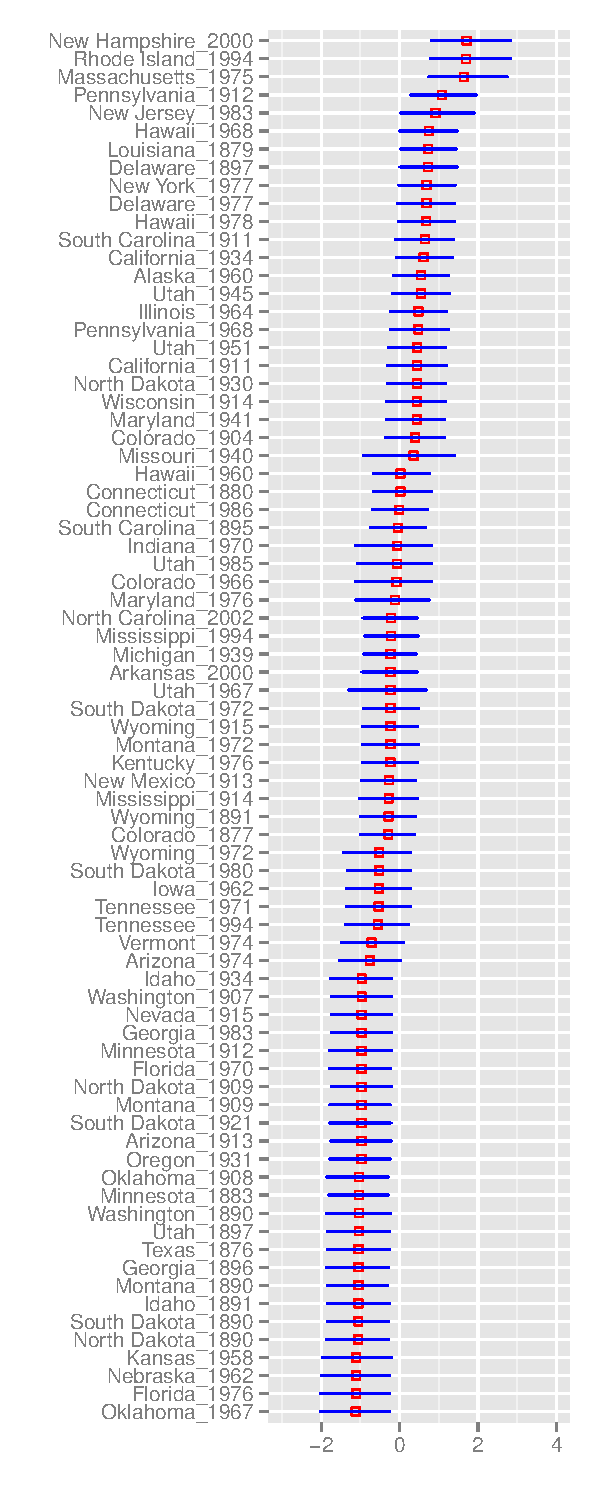
\includegraphics[height=\textheight]{graphics/regime/regime_param_mean_second_ggplot.pdf}
		\end{subfigure}
\end{figure}

%\singlespacing
%\bibliographystyle{apsr}
%\bibliography{measurementbib}	
\end{document}

